\section{Моделювання}

\subsection{Процес Пуассона}
Щоб моделювати темп виконання студентами контрольних задач, скористуємося
відомими з психології даними щодо ритму виконання теппінг-тесту для людей
з різними типами вищої нервової діяльності.
Оскільки постукування є потоком однорідних випадкових подій, змоделюємо їх
як реалізації процесу Пуассона.

Нехай $\left\{ N\left( t \right) \vert t \ge 0 \right\}$ --- процес Пуассона з
інтенсивністю $\lambda\left( t \right)$.
Маємо $7$ контрольних точок на часовій вісі $t_0 = 0, t_1 = 5, \dots, t_6 = 30$.
Введемо відрізок часу $T$, за який проводиться вимірювання,
та проміжки $T_i$, на які його розбито в експерименті
\begin{equation*}
  T = \left( 0, 30 \right], \qquad
  T_i = \left( t_{i-1}, t_i \right], \qquad
  i = \overline{1, 6}
\end{equation*}
Нехай $\nu_i$ визначається наступним чином
\begin{equation*}
  \nu_i = N\left( t_i \right) - N\left( t_{i-1} \right),
  \qquad i = \overline{1,6}
\end{equation*}
Тоді $\nu_i$ --- випадкова величина, що має розподіл Пуассона з параметром
$\lambda_i$, де \cite{Bulinsky:2003}
\begin{equation*}
  \lambda_i
  = m\left( T_i \right)
  = \int\limits_{t_{i-1}}^{t_i} \lambda\left( \tau \right) \; d\tau, \qquad
  i = \overline{1, 6}
\end{equation*}
Функція $m$ --- міра інтенсивності. \cite{Kingman:1992}

Проміжки $T_i$ утворюють розбиття множини $T$, а отже не перетинаються.
Це означає, що випадкові величини $\nu_i$ незалежні між собою,
і є можливість згенерувати процес натискання за допомогою $6$ незалежних
випадкових величин, що мають розподіл Пуассона.

Відомо, що оцінка методу моментів є конзистентною, коли вона існує.
Тобто вибіркове середнє (перший вибірковий момент) є кращою оцінкою
математичного очікування (перший момент): немає іншої оцінки,
середньоквадратичне відхилення якої від математичного очікування менше,
ніж середньоквадратичне відхилення вибіркового середнього від математичного
очікування даної випадкової величини.

Інтенсивність (параметр $\lambda$) є математичним очікуванням випадкової
величини, що має розподіл Пуассона.
Маючи результати реальних експериментів, можна обчислити середні значення
кількості постукувань для кожного часового проміжку $T_i$, а отримані
результати використовувати в якості параметрів $\lambda_i$.

Візьмемо значення відомого експерименту з підручника \cite{Ilin:2001}, які
зображено на рис. \ref{fig:tapping:Ilin01}.
Оскільки результат один, то його значення будуть середніми з вибірки, що
складається з одного вектора --- їх і використаємо в якості параметрів
$\lambda_i$.
На рис. \ref{fig:tapping:poisson} зображено різні реалізації послідовності
випадкових величин, що розподілені за законом Пуассона з параметрами
\begin{equation*}
  \left[ \lambda_{1}, \lambda_{2}, \lambda_{3}, \lambda_{4}, \lambda_{5},
         \lambda_{6} \right]
  = \left[ 43, 40, 38, 37, 38, 35 \right]
\end{equation*}

\begin{figure}[h]
  \centering
    \begin{tikzpicture}[scale=1]
      \begin{axis}[ymin=20, ymax=50, xmin=5, xmax=30, ytick=\empty,
        xmajorgrids={true},
        ylabel={Кількість точок}, ylabel near ticks,
        xlabel={час, с}]

        \draw[dashed,color=gray!50] ({rel axis cs:0,43}|-{axis cs:0,43})
                                 -- ({rel axis cs:1,43}|-{axis cs:0,43});
        \addplot table [x, y, col sep=comma] {data/chartIlinExample01.csv};
      \end{axis}
    \end{tikzpicture}
  \caption{Спадна ламана, побудована на основі даних з книги Ільїна}
  \label{fig:tapping:Ilin01}
\end{figure}

\subsection{Квадратична апроксимація}

Види результуючих ламаних (опукла, ввігнута, рівна, спадна) можна представити
квадратичними функціями виду
\begin{equation*}
  y\left( t \right) = a \cdot t^2 + b \cdot t + c
\end{equation*}

На рис. \ref{fig:tapping:poisson:sqr} зображено реалізації послідовності
випадкових величин, що розподілені за законом Пуассона, та криві, що є
результатом апроксимації цих реалізацій.

\begin{figure}[h]
  \centering
  \begin{subfigure}[b]{0.45\textwidth}
    %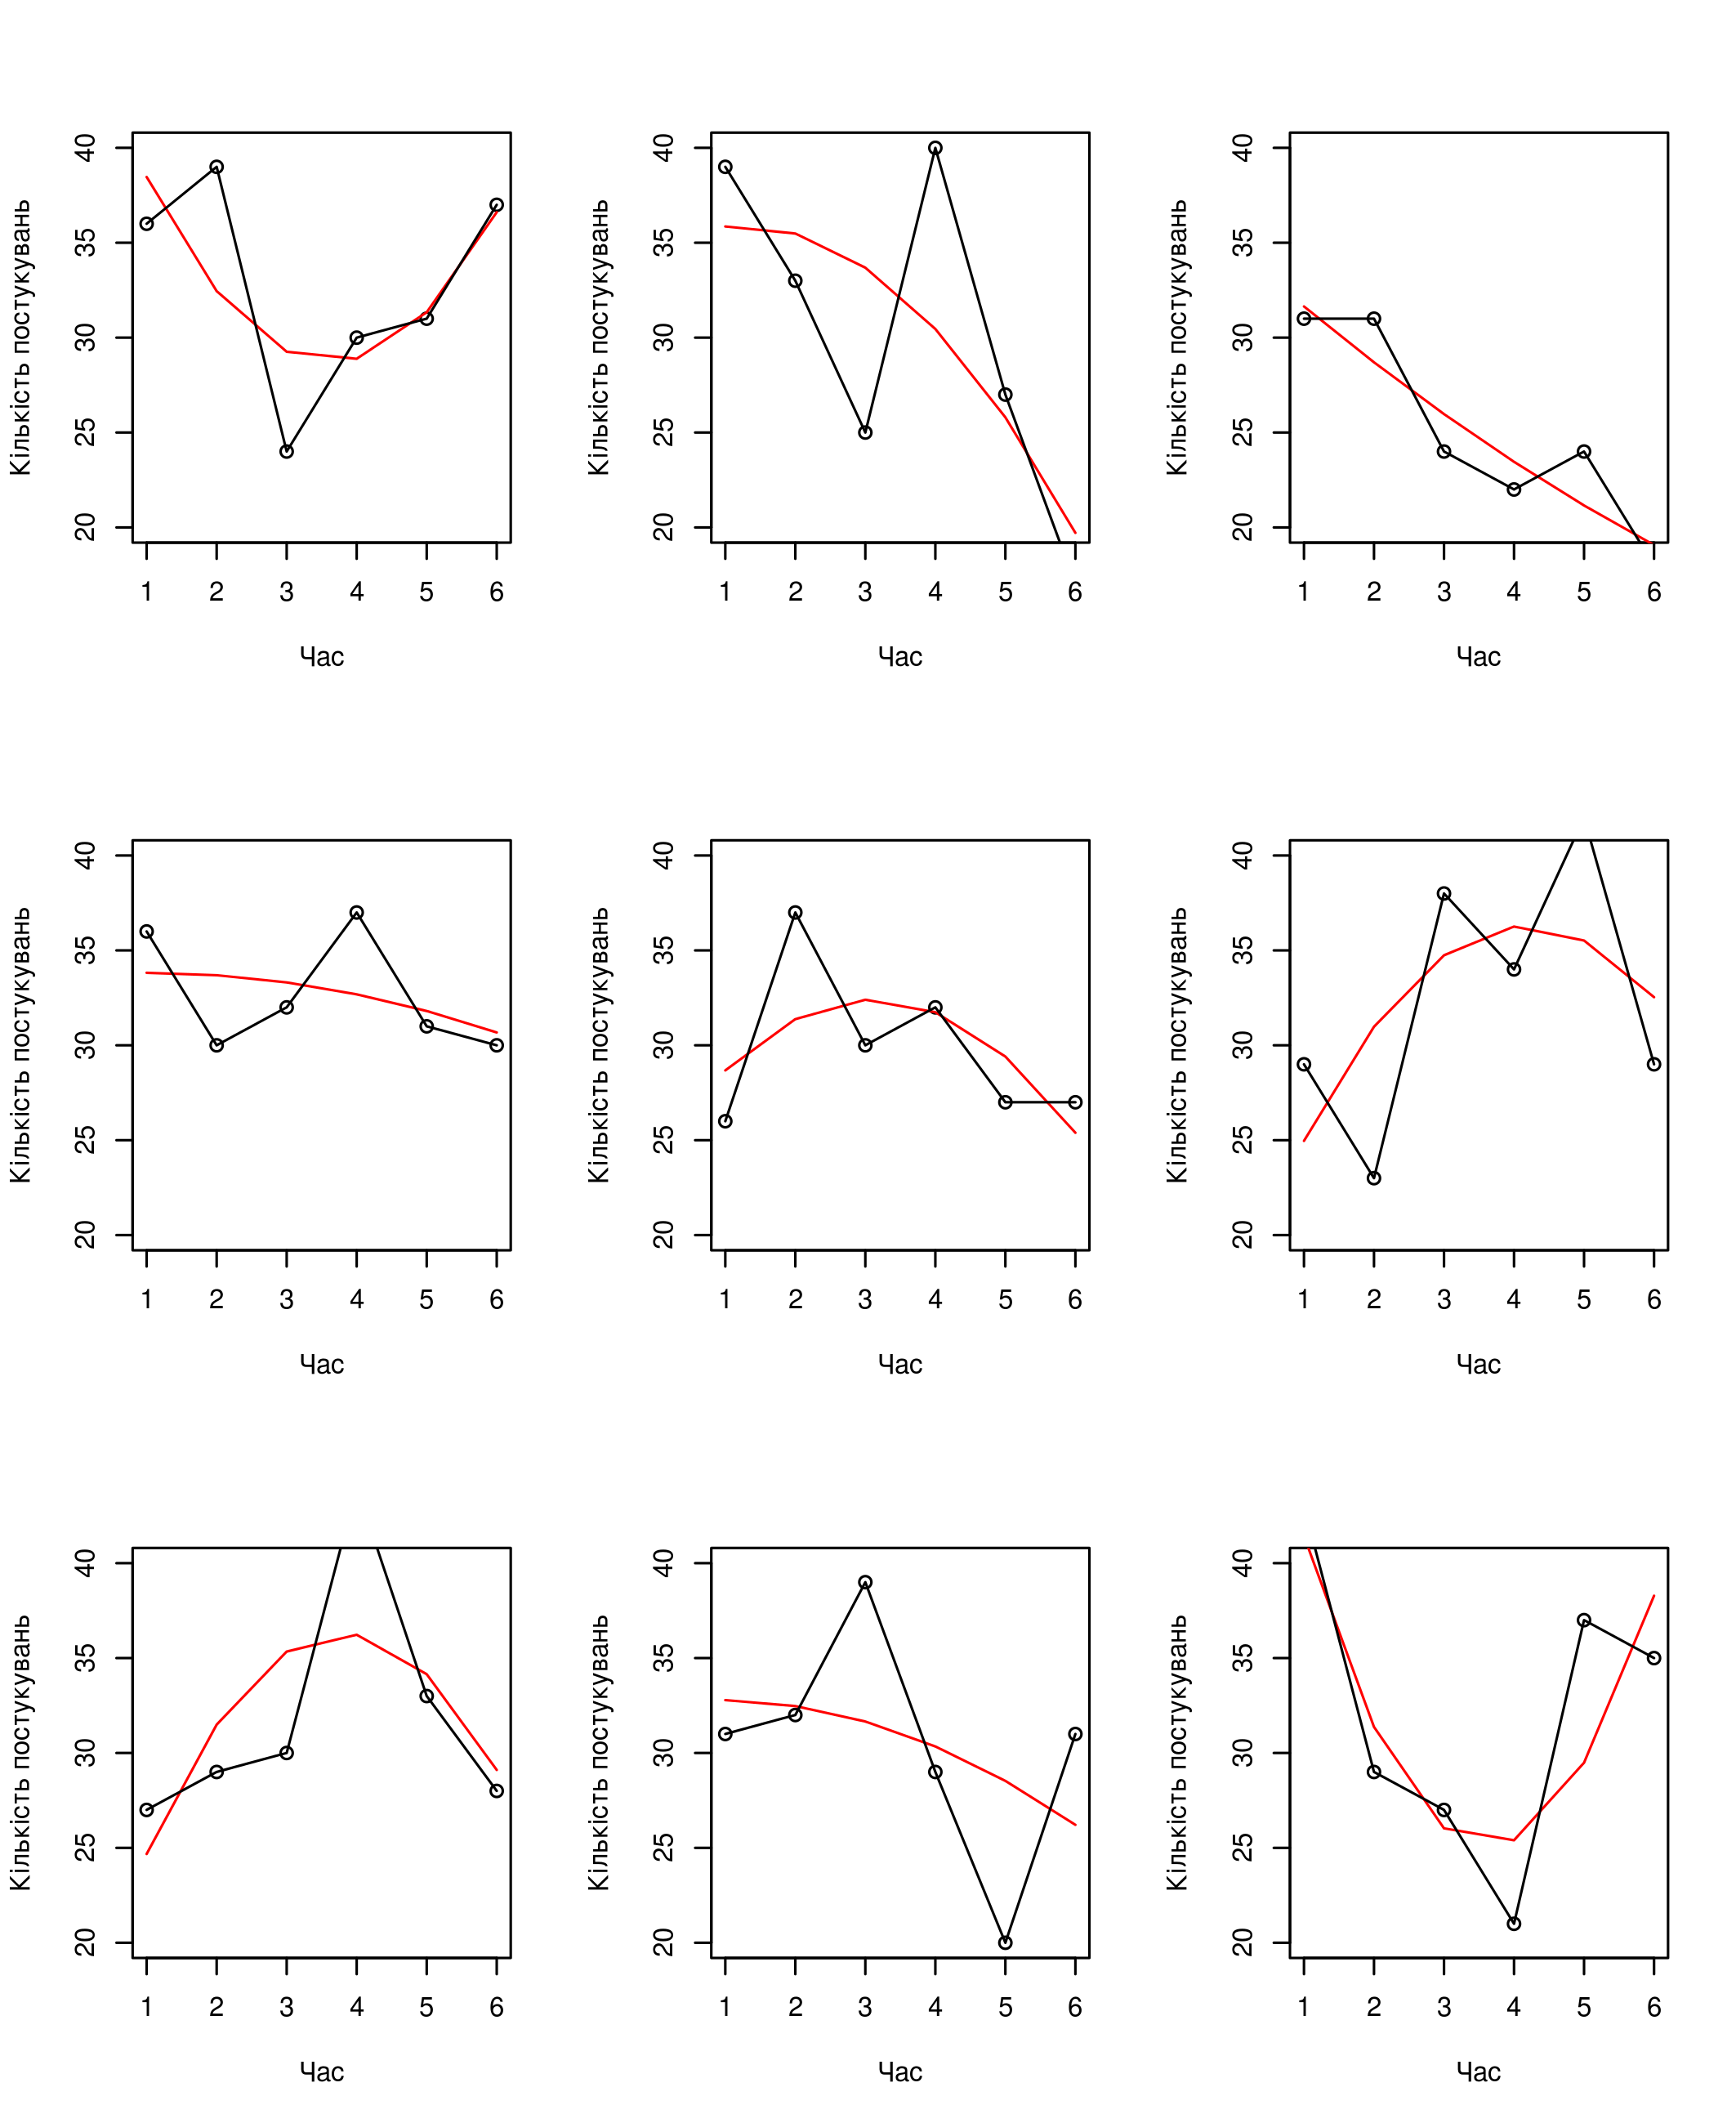
\includegraphics[width=.75\textwidth]{code/least_squares_approximation}
    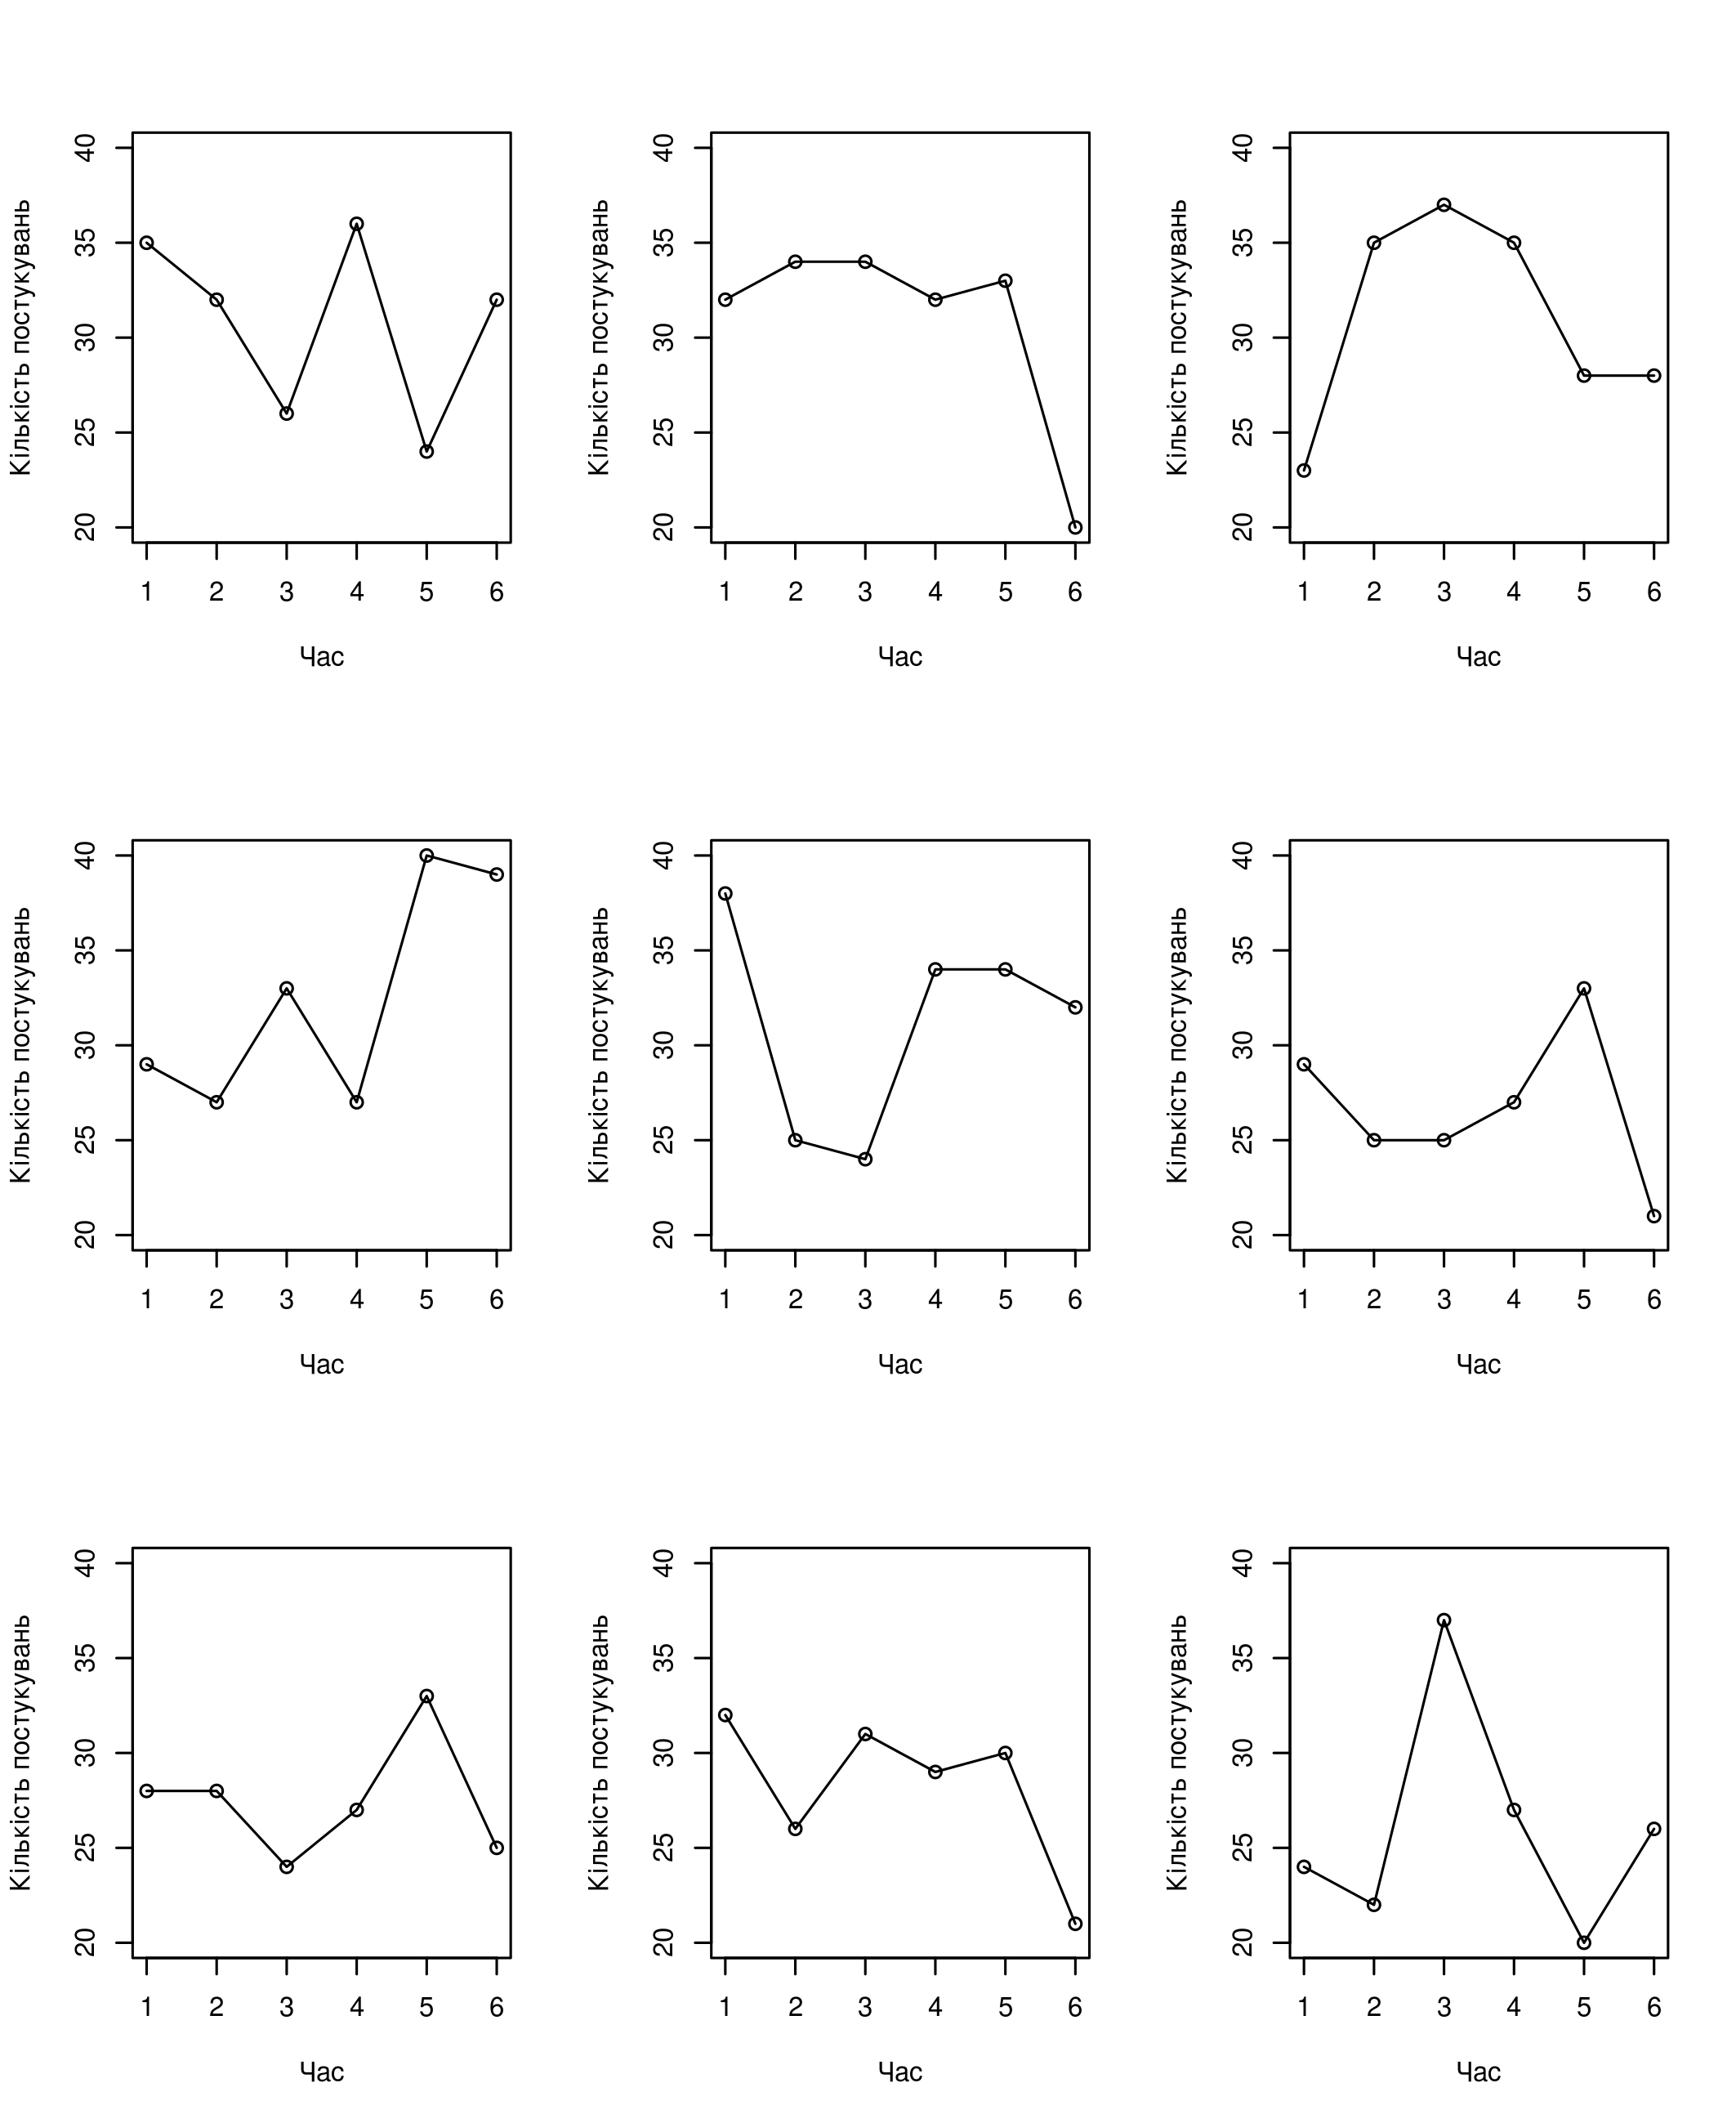
\includegraphics[width=\textwidth]{code/example_2.png}
    \caption{Без апроксимації}
    \label{fig:tapping:poisson}
  \end{subfigure}
  \begin{subfigure}[b]{0.45\textwidth}
    %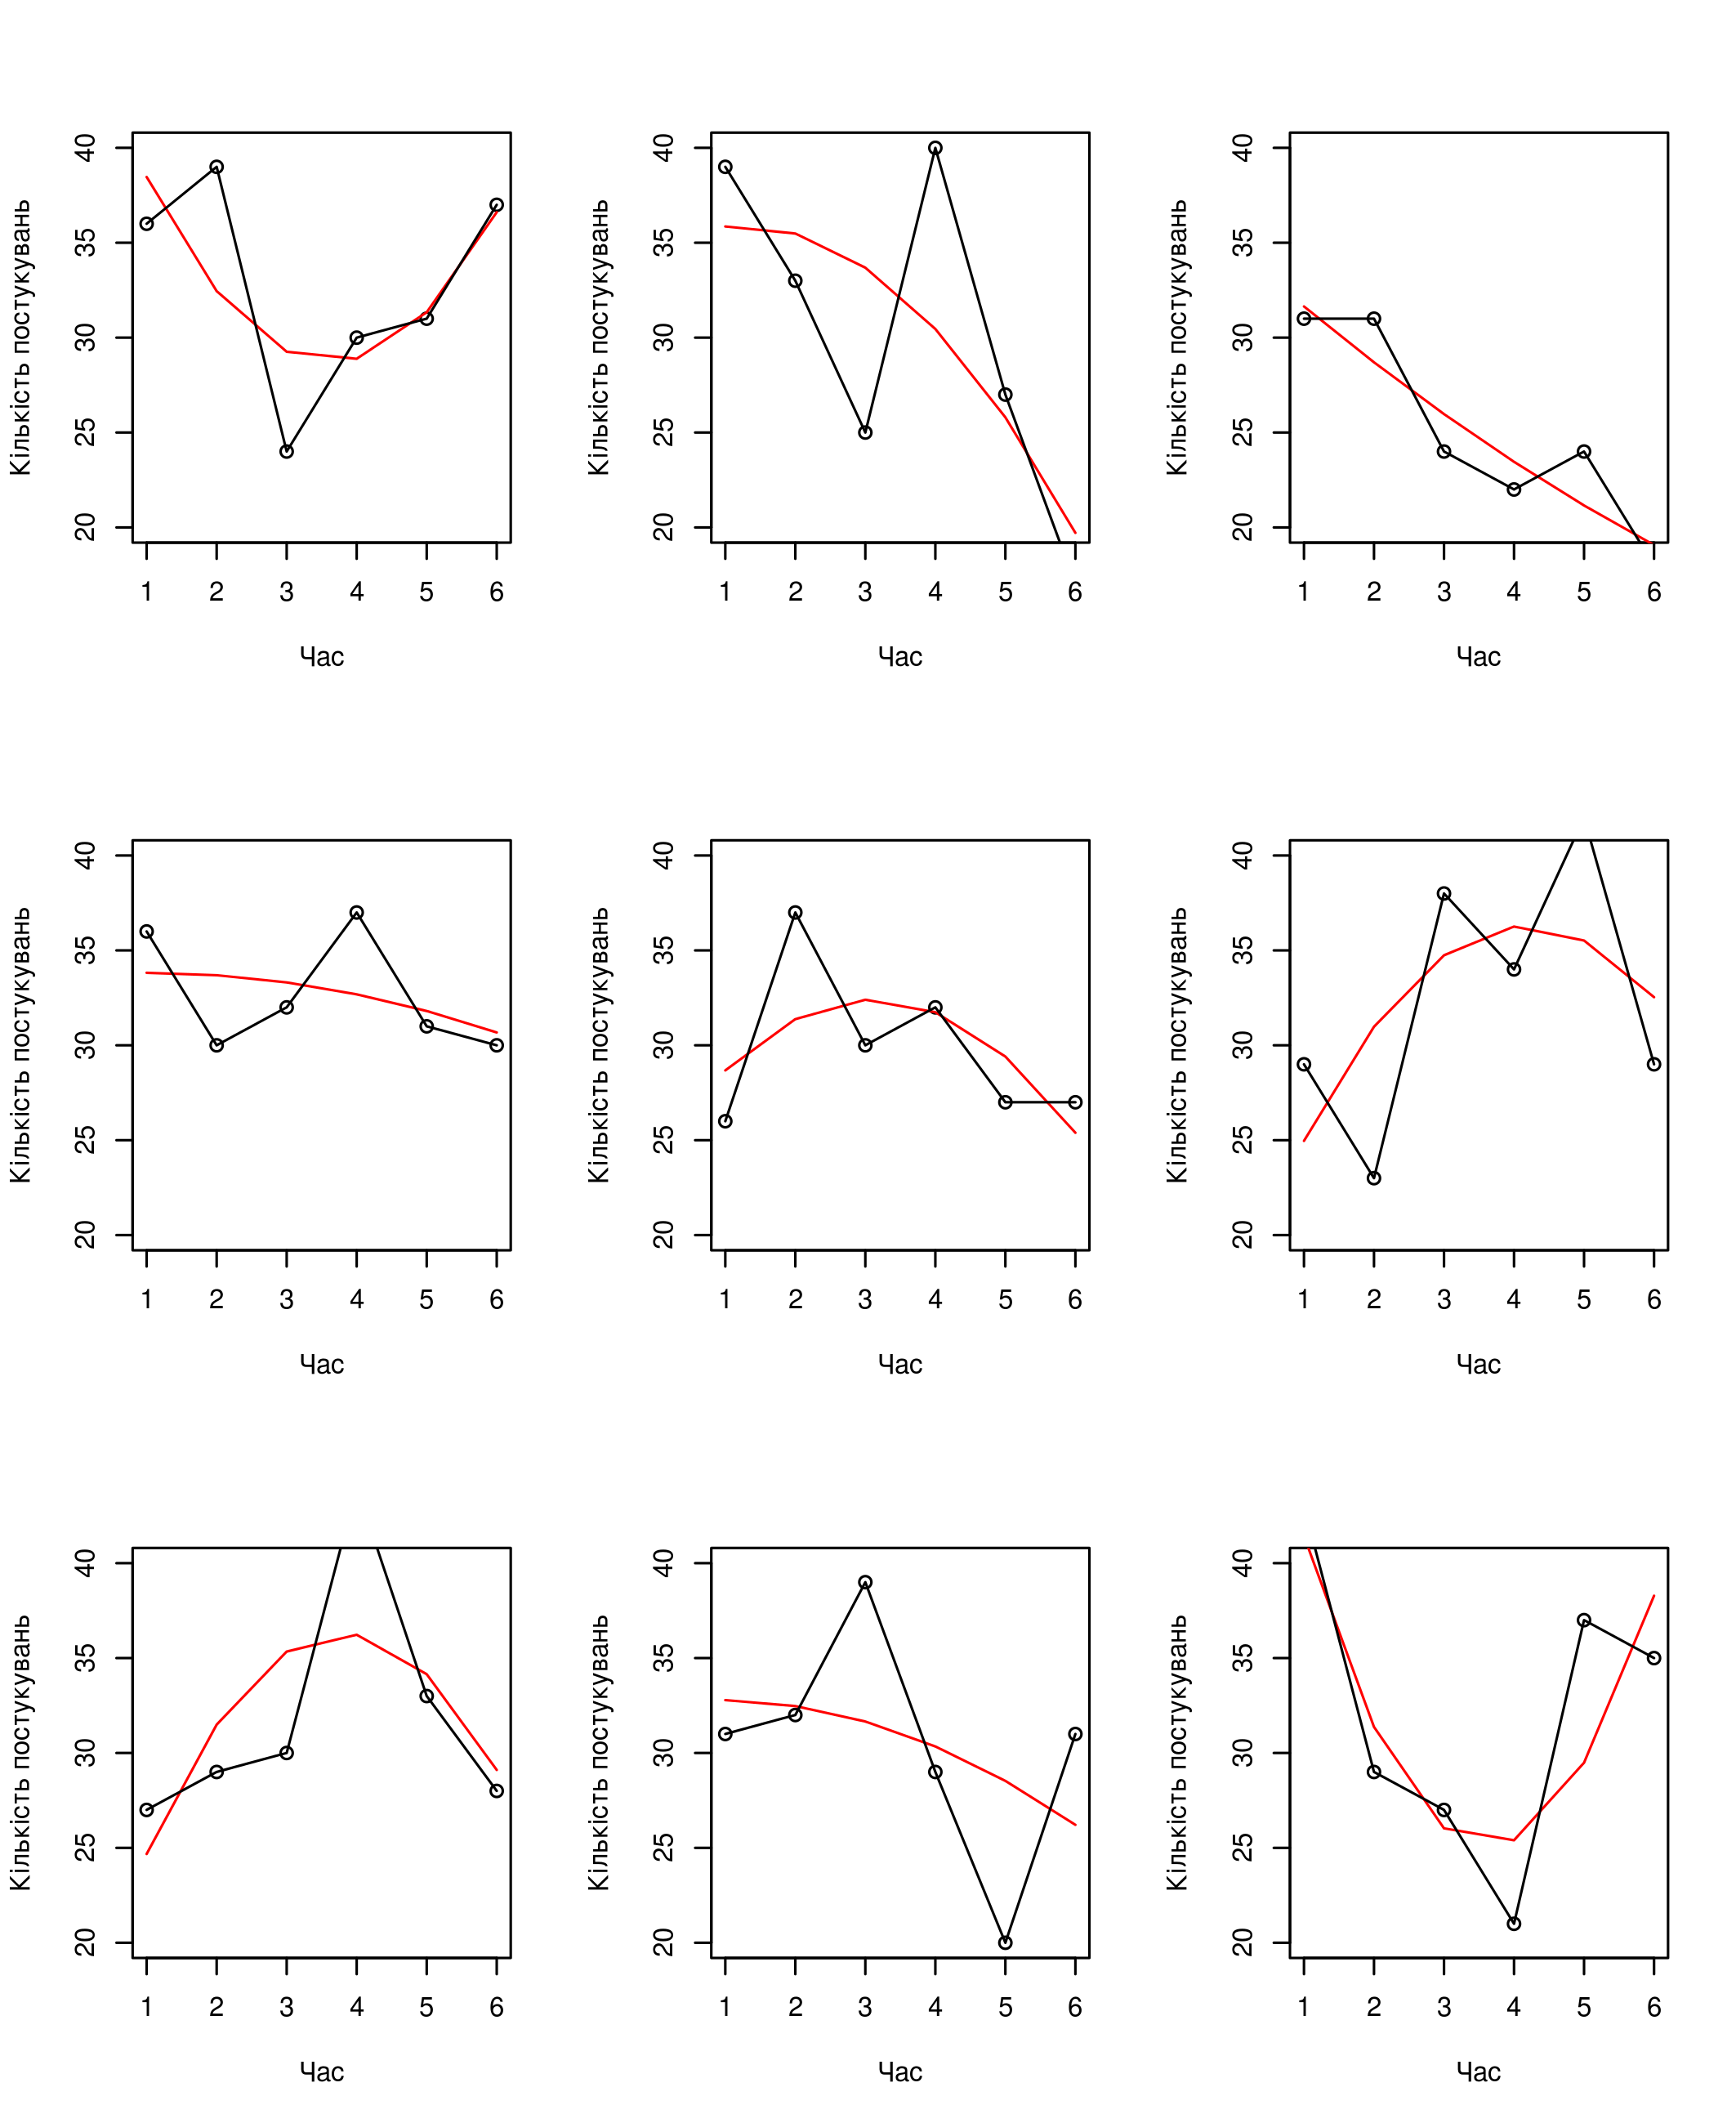
\includegraphics[width=.75\textwidth]{code/least_squares_approximation}
    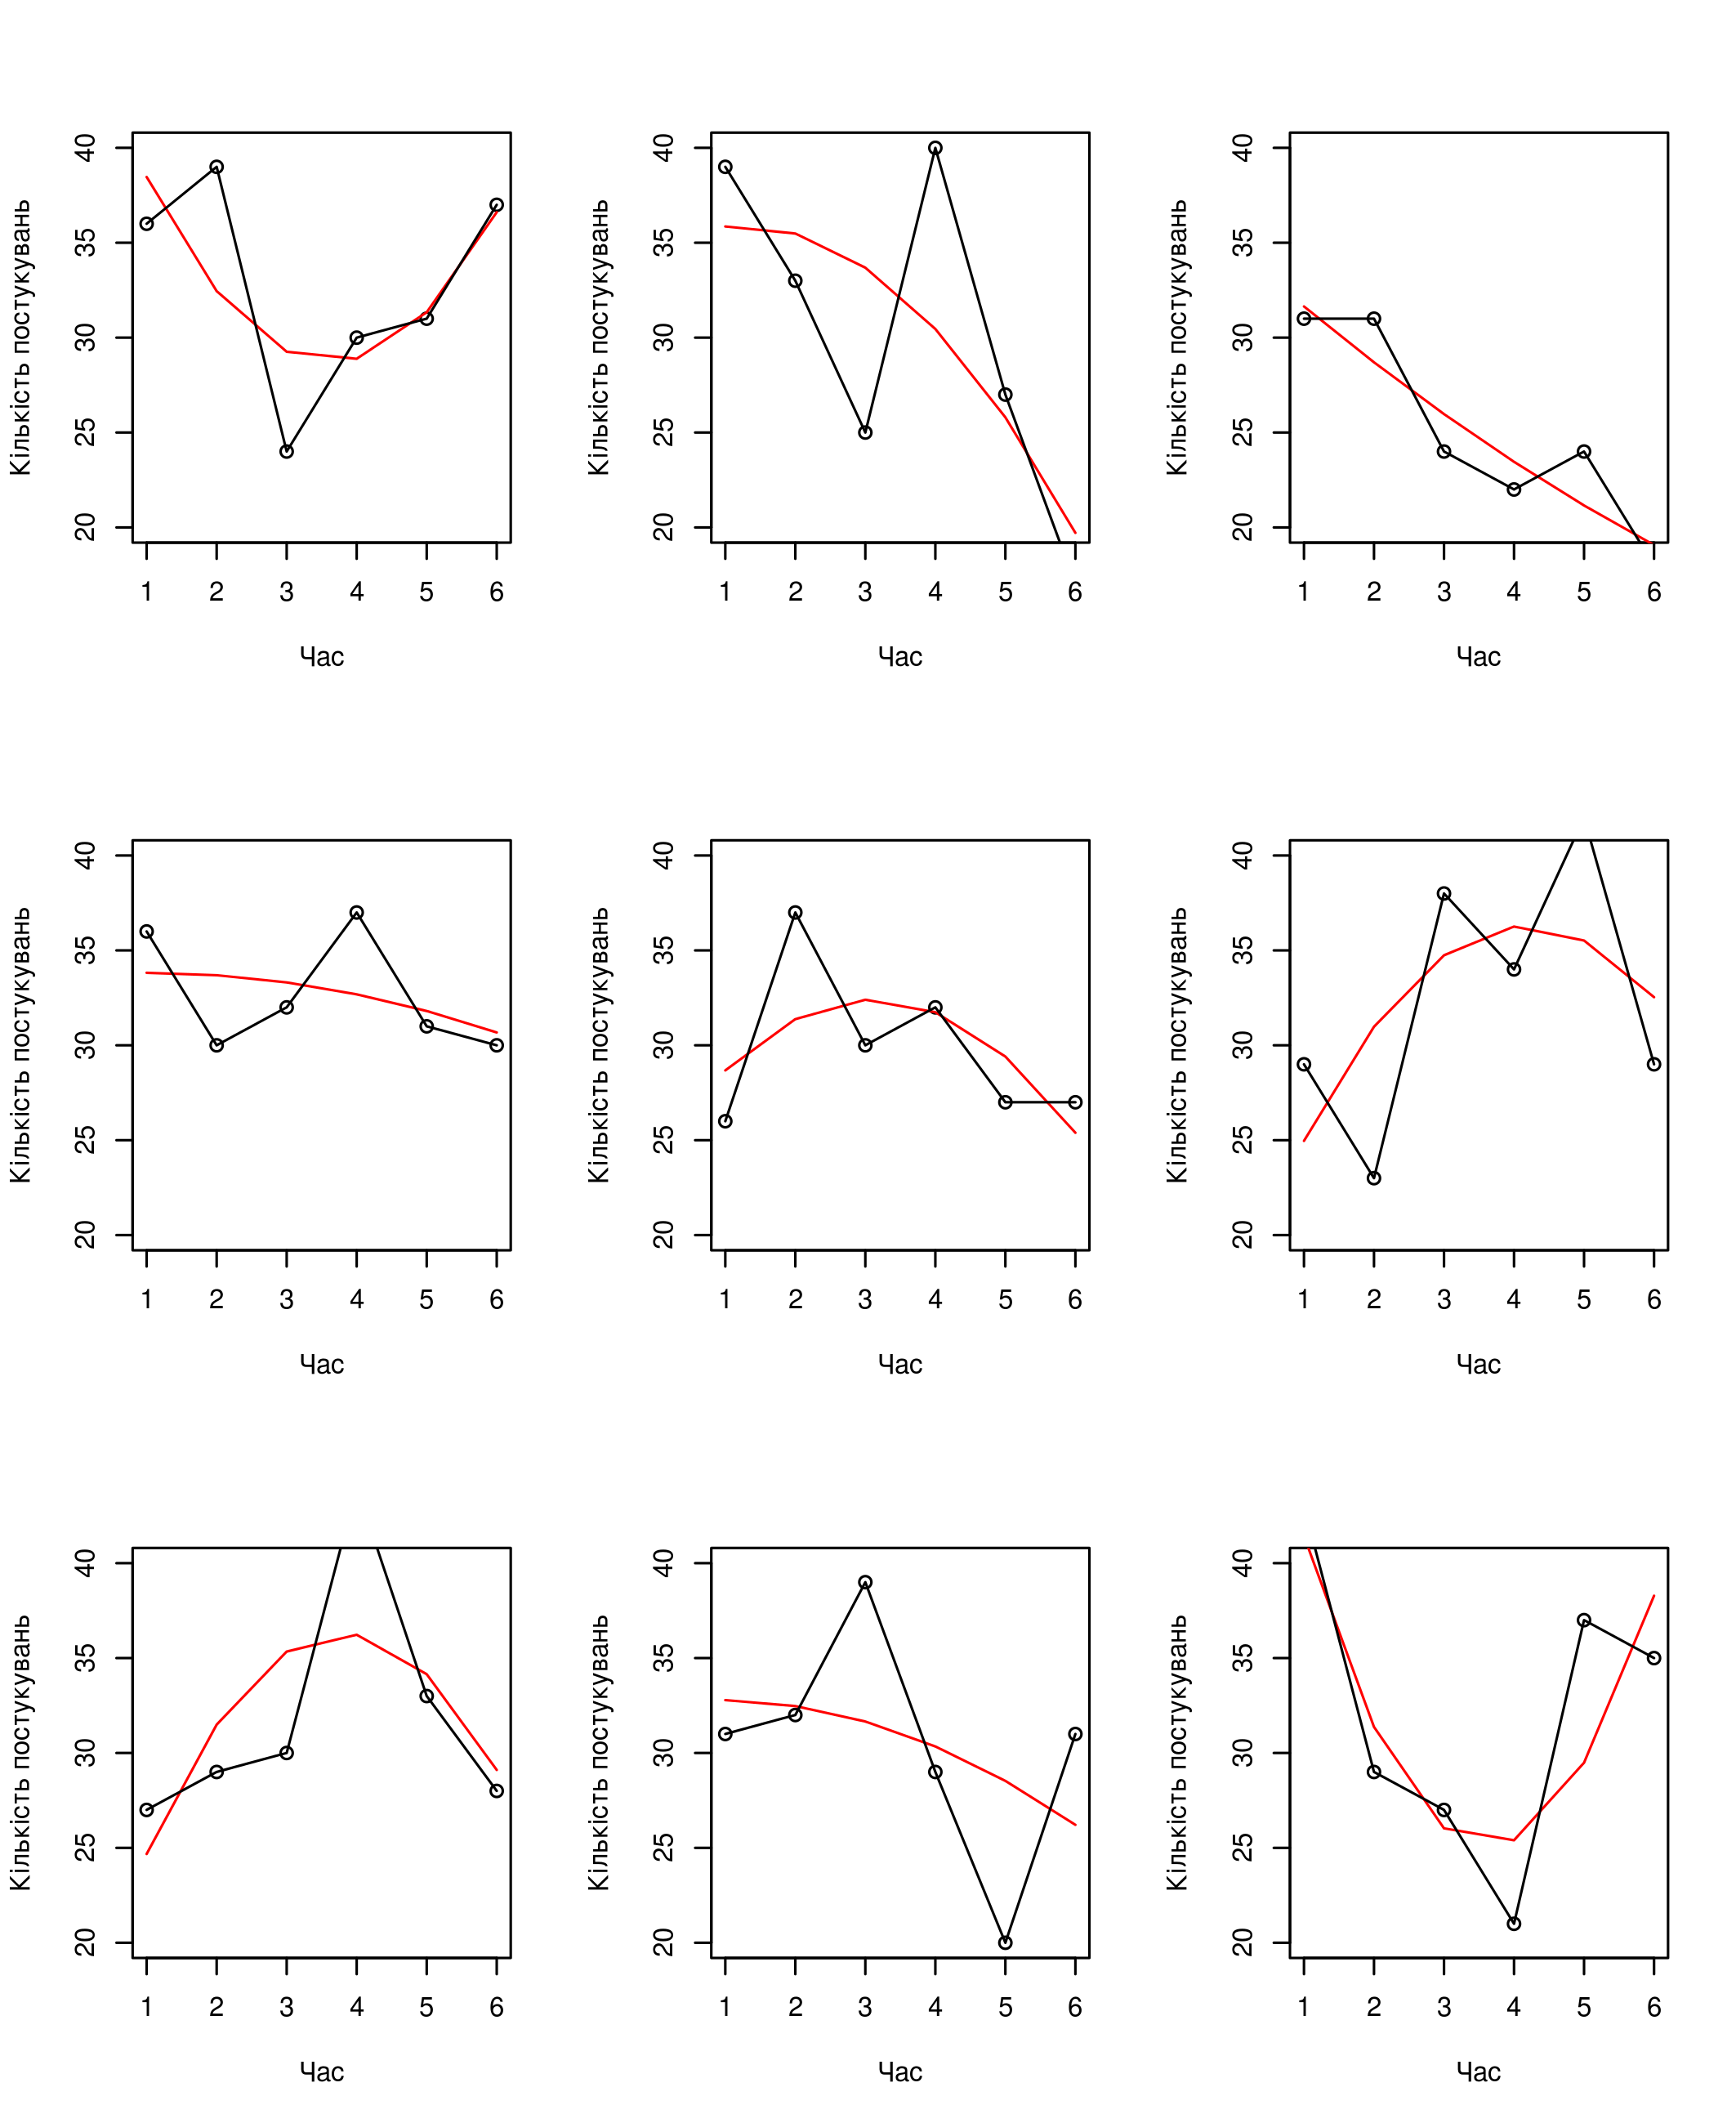
\includegraphics[width=\textwidth]{code/least_squares_approximation}
    \caption{З апроксимацією}
    \label{fig:tapping:poisson:sqr}
  \end{subfigure}
  \caption{Приклади результатів моделювання}
\end{figure}

\subsubsection{Метод найменших квадратів}
Щоб представити результати у вигляді квадратичних функцій, скористаємось
методом найменших квадратів.
Нехай $\left\{ y_i \mid i=\overline{1, 6} \right\}$ --- результати поточного
тепінг-тесту.
Суть методу полягає в знаходженні таких коефіцієнтів $a$, $b$ і $c$, з якими
наступна сума приймає мінімальне значення
\begin{equation*}
  R^2\left( a, b, c \right)
  = \sum_{i=1}^{6} \left( a \cdot t_i^2 + b \cdot t_i + c - y_i \right)^2
\end{equation*}
Для цього треба взяти часткові похідні по кожному коефіцієнту, прирівняти ці
похідні до нуля та розв’язати отримане рівняння
\begin{equation*}
  \begin{cases}
    \sum_{i=1}^{6} 2 \cdot \left( a \cdot t_i^2 + b \cdot t_i + c - y_i \right)
    &= 0 \\
    \sum_{i=1}^{6} 2 \cdot t_i
      \cdot \left( a \cdot t_i^2 + b \cdot t_i + c - y_i \right)
    &= 0 \\
    \sum_{i=1}^{6} 2 \cdot t_i^2
      \cdot \left( a \cdot t_i^2 + b \cdot t_i + c - y_i \right)
    &= 0 \\
  \end{cases}
\end{equation*}
Цю систему можна переписати в матричному вигляді наступним чином
\begin{equation*}
  \begin{bmatrix}
    \sum_{i=1}^{6} t_i^2 & \sum_{i=1}^{6} t_i   & \sum_{i=1}^{6} i \\
    \sum_{i=1}^{6} t_i^3 & \sum_{i=1}^{6} t_i^2 & \sum_{i=1}^{6} t_i \\
    \sum_{i=1}^{6} t_i^4 & \sum_{i=1}^{6} t_i^3 & \sum_{i=1}^{6} t_i^2
  \end{bmatrix}
  \cdot
  \begin{bmatrix}
    a \\
    b \\
    c
  \end{bmatrix}
  =
  \begin{bmatrix}
    \sum_{i=1}^{6} y_i \\
    \sum_{i=1}^{6} y_i \cdot t_i \\
    \sum_{i=1}^{6} y_i \cdot t_i^2
  \end{bmatrix}
\end{equation*}
Введемо позначення:
\begin{equation*}
  \begin{split}
    &\sum_{i=1}^{6} i = N, \\
    &\sum_{i=1}^{6} t_i^k = X^k,\qquad k=\overline{1, 4} \\
    &\sum_{i=1}^{6} y_i \cdot t_i^k = YX^k,\qquad k=\overline{0, 2}
  \end{split}
\end{equation*}
Рівняння прийняло наступний вигляд
\begin{equation*}
  \begin{bmatrix}
    X^2 & X   & N \\
    X^3 & X^2 & X \\
    X^4 & X^3 & X^2
  \end{bmatrix}
  \cdot
  \begin{bmatrix}
    a \\
    b \\
    c
  \end{bmatrix}
  =
  \begin{bmatrix}
    Y \\
    YX \\
    YX^2
  \end{bmatrix}
\end{equation*}
Скористуємось методом Крамера.
Визначник $\Delta$
\begin{equation*}
  \begin{split}
    \Delta
    = X^2 \cdot \left( X^2 \cdot X^2 - X  \cdot X^3 \right)
       &- X \cdot \left( X^3 \cdot X^2 - X  \cdot X^4 \right) \\
       &+ N \cdot \left( X^3 \cdot X^3 - X^2 \cdot X^4 \right)
  \end{split}
\end{equation*}
Визначник $\Delta_a$
\begin{equation*}
  \begin{split}
    \Delta_a
    =     Y   \cdot \left( X^2 \cdot X^2 - X \cdot X^3 \right)
      &- YX   \cdot \left( X   \cdot X^2 - N \cdot X^3 \right) \\
      &+ YX^2 \cdot \left( X   \cdot X   - N \cdot X^2 \right)
  \end{split}
\end{equation*}
Визначник $\Delta_b$
\begin{equation*}
  \begin{split}
    \Delta_b
    =  -  Y   \cdot \left( X^3 \cdot X^2 - X \cdot X^4 \right)
      &+ YX   \cdot \left( X^2 \cdot X^2 - N \cdot X^4 \right) \\
      &- YX^2 \cdot \left( X^2 \cdot X   - N \cdot X^3 \right)
  \end{split}
\end{equation*}
Визначник $\Delta_c$
\begin{equation*}
  \begin{split}
    \Delta_c
    =     Y   \cdot \left( X^3 \cdot X^3 - X^2 \cdot X^4 \right)
      &- YX   \cdot \left( X^2 \cdot X^3 - X   \cdot X^4 \right) \\
      &+ YX^2 \cdot \left( X^2 \cdot X^2 - X   \cdot X^3 \right)
  \end{split}
\end{equation*}
Відомо, що розв’язками є наступні вирази
\begin{equation*}
  a = \frac{\Delta_a}{\Delta},\qquad
  b = \frac{\Delta_b}{\Delta},\qquad
  c = \frac{\Delta_c}{\Delta}
\end{equation*}
Також бачимо, що всі параметри лінійно залежать від усіх $y_i$.
Тобто можна записати розв’язки наступним чином
\begin{equation*}
  a = \sum_{i=1}^{6} y_i \cdot a_i,\qquad
  b = \sum_{i=1}^{6} y_i \cdot b_i,\qquad
  c = \sum_{i=1}^{6} y_i \cdot c_i
\end{equation*}

\subsubsection{Аналіз апроксимації}

Знайдемо умови, що накладаються на $a$, $b$ і $c$, за якиих отримана
парабола відповідає раніше введеним типам вищої нервової діяльності.
